\documentclass[aspectratio=169]{beamer}
\usetheme{Madrid}
\usecolortheme{whale}
\usepackage{booktabs}
\usepackage{graphicx}
\graphicspath{{../figures/}}

\definecolor{cainiao}{HTML}{0571B0}
\setbeamercolor{structure}{fg=cainiao}
\setbeamertemplate{navigation symbols}{}
\setbeamertemplate{caption}{\raggedright\insertcaption\par}

\title[Cainiao is Fast --- But Not Everywhere]{Cainiao is Fast --- But Not Everywhere}
\subtitle{When does Alibaba's logistics network stop delivering its speed advantage?}
\author{Group 12}
\institute{BUAD 345: Decision Analytics and Visualization}
\date{Summer 2026}

\begin{document}

\begin{frame}[plain]
  \titlepage
\end{frame}

% 1
\begin{frame}{The question}
  \begin{itemize}
    \item \textbf{Audience: Cainiao} (Alibaba's logistics platform).
    \item Delivery speed drives sales and loyalty: online sales rise $\sim$1.45\%
          per business-day faster delivery (Fisher et al., 2019); late delivery
          erodes loyal customers (Rao et al., 2011).
    \item Cainiao handles \textbf{30.2\%} of orders --- does it actually deliver
          faster, and \emph{everywhere}?
  \end{itemize}
  \vfill
  \footnotesize Data: 1.29M Tmall orders, Jan--Jul 2017 (order + 969\,MB logistics
  + merchant files).
\end{frame}

% 2
\begin{frame}{Method: dig hierarchically, not in parallel}
  \[
    \text{totaltime} = \text{SIGNED} - \text{pay\_timestamp}\ (\text{hours})
  \]
  \begin{enumerate}
    \item Cainiao vs.\ non-Cainiao
    \item $+$ carrier size (Large $>$200k orders)
    \item $+$ destination-city size (top-2 signing cities = Big)
    \item segment decomposition: pre-delivery / line-haul / last-mile
  \end{enumerate}
  \vfill
  \footnotesize One focused theme; each level added only when the previous result
  motivates it.
\end{frame}

% 3
\begin{frame}{Headline: Cainiao is faster overall}
  \begin{columns}
    \begin{column}{0.52\textwidth}
      \begin{itemize}
        \item \textbf{61.9\,h} vs.\ \textbf{71.0\,h} $\Rightarrow$ $\sim$9.2\,h faster.
        \item Survives a fair control: among no-promise orders, 62.5 vs.\ 71.0\,h.
        \item Stable across the whole 7-month window.
      \end{itemize}
    \end{column}
    \begin{column}{0.46\textwidth}
      \centering
      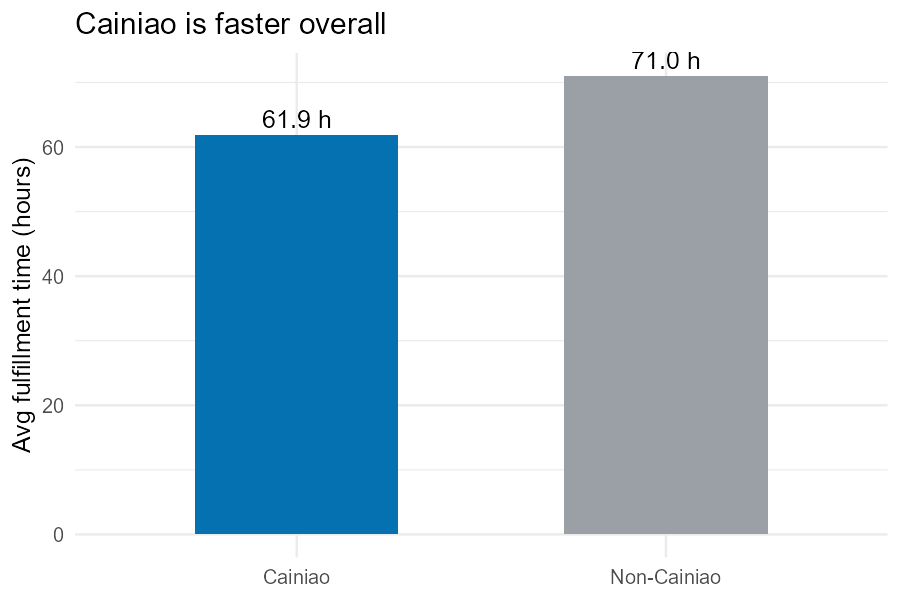
\includegraphics[width=\textwidth]{fig1_main_effect.png}
    \end{column}
  \end{columns}
\end{frame}

% 4
\begin{frame}{Stable over time}
  \centering
  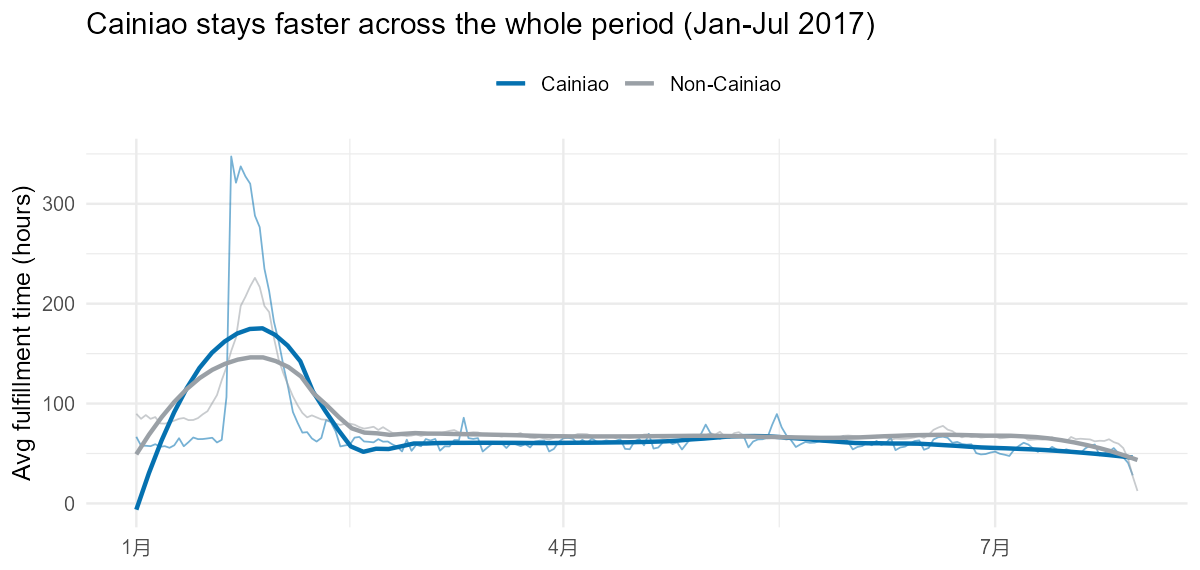
\includegraphics[width=0.86\textwidth]{fig5_daily_trend.png}
\end{frame}

% 5
\begin{frame}{...BUT the advantage is uneven --- the punchline}
  \centering
  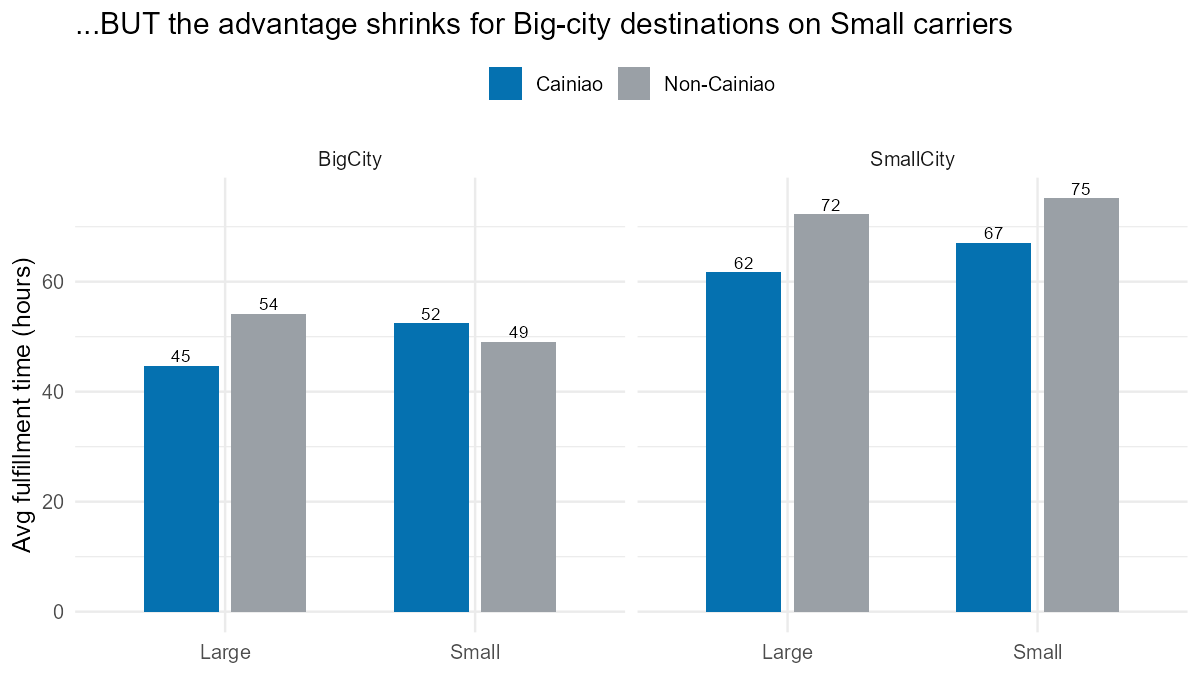
\includegraphics[width=0.82\textwidth]{fig2_punchline.png}

  \footnotesize For \textbf{big-city destinations on small carriers}, Cainiao is
  \textcolor{red}{3.3\,h \emph{slower}} than non-Cainiao.
\end{frame}

% 6
\begin{frame}{The reversal cell, in numbers}
  \centering
  \begin{tabular}{llrrr}
    \toprule
    Destination & Carrier & Cainiao & Non-Cainiao & \textbf{Cainiao saved} \\
    \midrule
    Big city   & Large & 44.7 & 54.2 & \textbf{+9.5\,h} \\
    Big city   & Small & 52.4 & 49.1 & \textbf{\textcolor{red}{$-$3.3\,h}} \\
    Small city & Large & 61.7 & 72.2 & \textbf{+10.5\,h} \\
    Small city & Small & 67.1 & 75.2 & \textbf{+8.0\,h} \\
    \bottomrule
  \end{tabular}
  \vfill
  \footnotesize 22{,}756 orders in the reversal cell --- not a small-sample fluke.
\end{frame}

% 7
\begin{frame}{Customers feel it too}
  \centering
  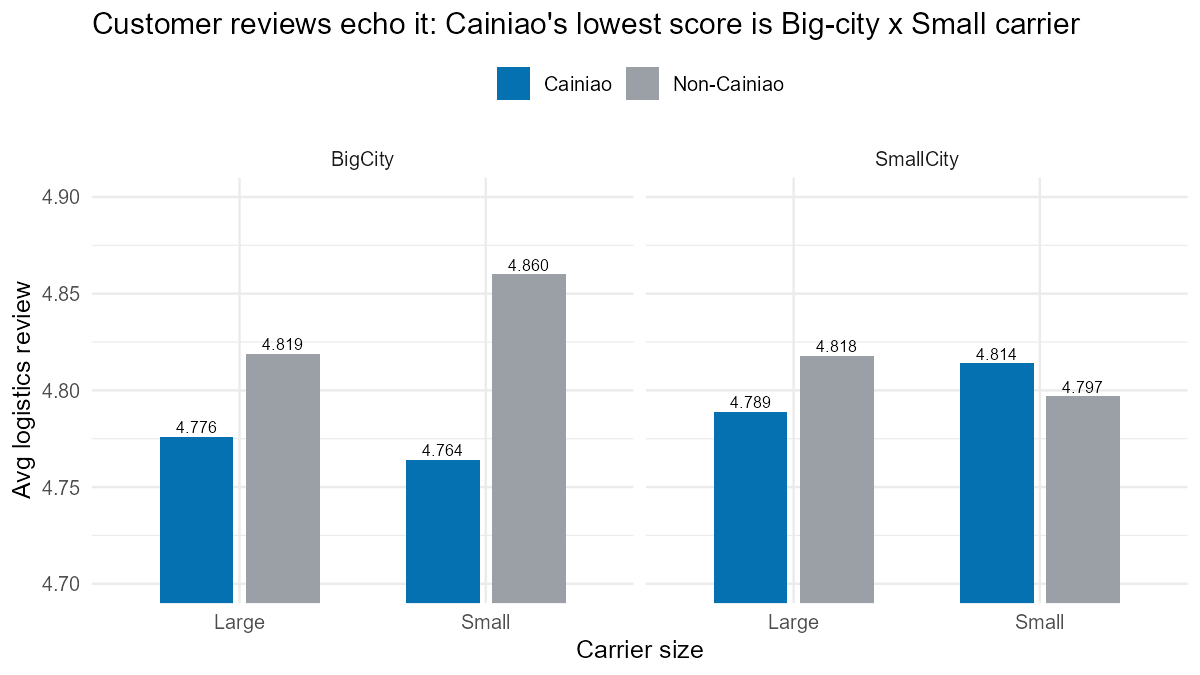
\includegraphics[width=0.8\textwidth]{fig4_review.png}

  \footnotesize Cainiao's \emph{lowest} review (4.764) is the same big-city /
  small-carrier cell; non-Cainiao's \emph{highest} (4.860) is right beside it.
\end{frame}

% 8
\begin{frame}{Mechanism: it's line-haul, not the last mile}
  \begin{columns}
    \begin{column}{0.5\textwidth}
      \begin{itemize}
        \item Last-mile is small \& similar everywhere ($\sim$4--6\,h).
        \item Cainiao's edge = faster \textbf{line-haul}
              (e.g.\ 38.4 vs.\ 47.8\,h).
        \item In the reversal cell that edge vanishes (27.0 vs.\ 26.9\,h).
      \end{itemize}
    \end{column}
    \begin{column}{0.5\textwidth}
      \centering
      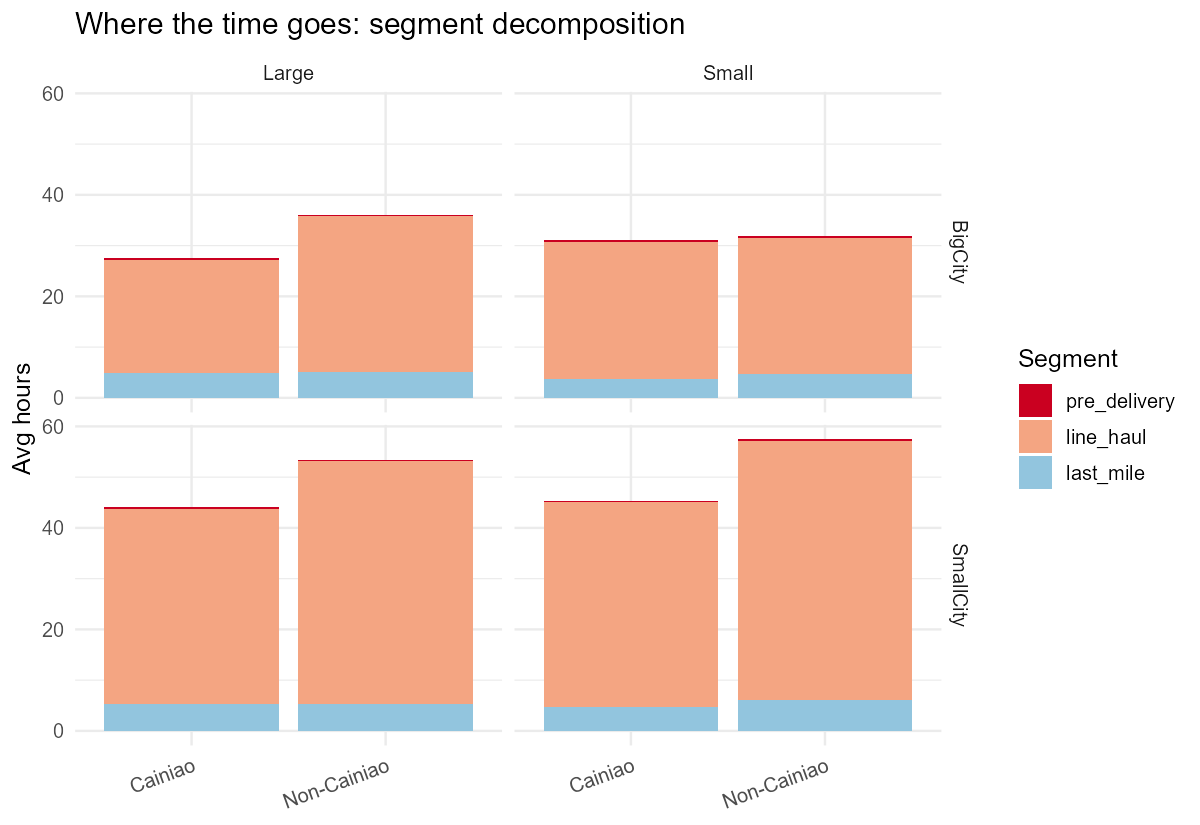
\includegraphics[width=\textwidth]{fig3_segments.png}
    \end{column}
  \end{columns}
\end{frame}

% 9
\begin{frame}{An honest non-result}
  \begin{itemize}
    \item Hypothesis: small carriers make more stops $\Rightarrow$ slower.
    \item \textbf{Not supported.} Small carriers pass through \emph{fewer} cities
          (2.9--3.1) than large ones (3.4--3.7).
    \item So the penalty is \emph{per-leg} transit/dwell time, not more hops ---
          which sharpens the explanation we give.
  \end{itemize}
\end{frame}

% 10
\begin{frame}{Why}
  \begin{itemize}
    \item Big cities concentrate trunk-line volume; large carriers run dedicated,
          high-frequency line-haul, small carriers wait to consolidate
          (Yu et al., 2016).
    \item Small carriers can't execute one-size-fits-all smart routing; ignoring
          carrier heterogeneity degrades routing performance (Koç et al., 2016).
  \end{itemize}
\end{frame}

% 11
\begin{frame}{So what --- three moves for Cainiao}
  \begin{enumerate}
    \item \textbf{Deepen ties with large carriers} on big-city lanes (watch
          concentration risk).
    \item \textbf{Make smart-routing carrier-capability-aware} (size, coverage,
          experience).
    \item \textbf{Pilot big-city consolidation / parcel lockers} for small-carrier
          shipments to cut the line-haul + pickup penalty (Deutsch \& Golany, 2018).
  \end{enumerate}
  \vfill
  \footnotesize The weakness is concentrated, so the fix is cheap vs.\ a
  platform-wide change.
\end{frame}

% 12
\begin{frame}{Summary in two sentences}
  \begin{block}{Overall}
    Cainiao significantly shortens fulfillment time across the marketplace
    ($\sim$9\,h, robust to a promise control).
  \end{block}
  \begin{block}{Punchline}
    But that advantage largely disappears --- and reverses --- for big-city
    destinations served by small carriers, with the bottleneck in line-haul
    rather than the last mile.
  \end{block}
  \vfill
  \centering \footnotesize \emph{Limitations: observational data (association, not
  causation); missing milestones; coarse big-city proxy.}
\end{frame}

\begin{frame}[plain]
  \centering \Large Thank you --- Group 12 \\[0.5em]
  \normalsize Questions?
\end{frame}

\end{document}
